\documentclass[pdf, aspectratio=169, 12pt]{beamer}
\usepackage[]{hyperref, graphicx, siunitx, lmodern, tikz, booktabs, physics}
\usepackage[mode=buildnew]{standalone}
\usepackage{pdfpc-commands}
\usepackage{pgfplots}
\pgfplotsset{compat=1.16}

\usetheme[sols]{Python}

\graphicspath{ {Images/} }

\sisetup{per-mode=symbol}
\usetikzlibrary{calc, patterns, decorations.markings, decorations.pathmorphing, shapes}

%Preamble
\title{Showing some class}
\author{Jed Rembold}
\date{March 18, 2020}

\begin{document}

\begin{frame}{Announcements}
	\begin{itemize}
		\item HW5 graded and uploaded back to Github
		\item Midterm postponed!
			\begin{itemize}
				\item In light of everything, we are moving it back until the Friday you get back
				\item Will have a homework that week, so we'll figure out what that will look like.
			\end{itemize}
		\item Normal class day on Friday
		\item No lab today!
		\item I'll be getting updated grade-reports out during Spring Break
		\item Polling: \nolinkurl{rembold-class.ddns.net}
	\end{itemize}
\end{frame}

\begin{frame}[fragile]{Review Question}
	Which of the provided options would appear as below when printed? The sideways brackets are JUST to show you spaces. They would not appear!
	\begin{center}
		\pyi[output, showspaces=true]{101,234.98\ \ \ & 4000}
	\end{center}
	\begin{poll}
	\item \pyi{'\{:<12,f\} & \{:0>4d\}'.format(1.01234984e5, 320//8)}
	\item \pyi{'\{>12,.2f\} & \{0>4d\}'.format(1.01234984e5, 32000//8)}
	\item \pyi{'\{:<12,.2f\} & \{:<4d\}'.format(1.01234984e5, 3200//8)}
	\item \pyi{'\{:<12,.2f\} & \{:0<4d\}'.format(1.01234984e5, 32//8)}
	\end{poll}
	\exsol{\pyi{'\{:<12,.2f\} & \{:0<4d\}'.format(1.01234984e5, 32//8)}}
\end{frame}


\begin{frame}[fragile]{Ain't no g-string}
	\vspace{5mm}
	\begin{itemize}
		\item Short for format string, an f-string achieves the same thing as \pyi{.format} but with less syntax
		\item Introduced in Python 3.6
		\item Need an 'f' right before the string to let Python know it needs to do more with the string
		\item Place the desired variables (or values) directly into the \pyi{\{ \}}, where you'd normally have placed the label!
			\begin{pythoncode}
				A = 10
				B = 15.123234
				print(f'A is {A} and B is {B:.2f}')
			\end{pythoncode}
		\item All other syntax and format specs like \pyi{.format}!
	\end{itemize}
\end{frame}

\begin{frame}{Objectively\ldots}
	\begin{itemize}
		\item<+-> We've discussed many different kinds of data so far:
			\begin{center}
				\pyi{123}\hspace{1cm}\pyi{3.14}\hspace{1cm}\pyi{'Hello'}\hspace{1cm}\pyi{[2,4,6]}\\
				\pyi{True}\hspace{1cm}\pyi{(3,5,2)}\hspace{1cm}\pyi{\{'Apples':3, 'Bananas':6\}}
			\end{center}
			\vspace{5mm}
		\item<+-> Each is an \alert{object}, and every object has:
			\begin{itemize}
				\item a \emph{type}
				\item some form of internal \emph{data representation}
				\item a set of ways to \emph{interact} with the object
			\end{itemize}
		\item<+-> More particularly, an object is an \alert{instance} of some \emph{type}
			\begin{itemize}
				\item \pyi{True} is an instance of type \pyi{bool}
				\item \pyi{3.14159} is an instance of type \pyi{float}
			\end{itemize}
	\end{itemize}
\end{frame}

\begin{frame}{All the Objects}
	\begin{itemize}
		\item In Python, \textcolor{Red}{everything} is an object (and thus an instance of some type)
			\begin{itemize}
				\item Can \alert{create} new objects of some type
					\begin{itemize}
						\item \pyi{A = 'hello'}
					\end{itemize}
				\item Can \alert{manipulate} objects
					\begin{itemize}
						\item \pyi{A.lower()}
					\end{itemize}
				\item Can \alert{destroy} objects
					\begin{itemize}
						\item Can use \pyi{del} or reassign their label
						\item Python will clean up deleted or inaccessible objects
						\item Called \textcolor{Blue}{garbage collection}
					\end{itemize}
			\end{itemize}
	\end{itemize}
\end{frame}

\begin{frame}{What's my type?}
	\begin{itemize}
		\item When you think about it, a \alert{type} in Python encompasses two main ideas:
			\begin{enumerate}[<+->]
				\item It defines what the objects of that type \emph{are}. What properties it has. How it is represented internally in memory.
				\item It defines an \emph{interface} for how one interacts with objects of that type and how objects of that type interact with other objects.
			\end{enumerate}
	\end{itemize}
\end{frame}

\begin{frame}{Example: Lists}
	\begin{itemize}
		\item Consider the object \pyi{[2,4,6]} which has type \pyi{list}
		\item Has an \alert{internal representation} of two parts:
			\begin{itemize}
				\item A list of pointers to each of the element objects
				\item A value that keeps track of the allocated memory for the above list
			\end{itemize}
			\begin{center}
				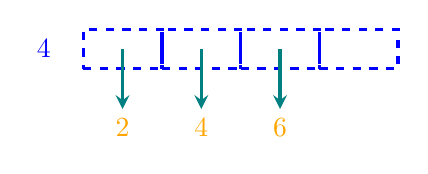
\begin{tikzpicture}
					\node[Blue] at (0,0) {4};
					\foreach \x in {1,2,3,4}{
						\node[draw, dashed, Blue, very thick, minimum width=1cm, minimum height=5mm](\x) at (\x,0) {};
					}
					\node[Orange](p2) at (1,-1) {2};
					\node[Orange](p4) at (2,-1) {4};
					\node[Orange](p6) at (3,-1) {6};
					\path[-stealth, very thick, Teal]
						(1.center) edge (p2)
						(2.center) edge (p4)
						(3.center) edge (p6);
				\end{tikzpicture}
			\end{center}
			\pause
		\item Has ways to \alert{manipulate} lists:
			\begin{itemize}
				\item \pyi{L[i]}, \pyi{L[i:j]}
				\item \pyi{len()}, \pyi{max()}, \pyi{del(L[i])}
				\item \pyi{L.append()}, \pyi{L.count()}, \pyi{L.remove()}, etc
				\item We use these methods instead of messing with the internal representation
			\end{itemize}
	\end{itemize}
\end{frame}

\begin{frame}{Object Oriented Programming}
	\begin{itemize}
		\item Object Oriented Programming is just a paradigm of making objects and their accompanying types the star of the show
		\item Python is setup nicely for this paradigm considering everything is already an object
		\item Advantages:
			\begin{itemize}
				\item Bundles data and procedures to operate on that data together in nice packages and with well defined interfaces
				\item Allows to implement and test different object types independently
				\item Modularity reduces complexity and makes it easy to reuse code
			\end{itemize}
	\end{itemize}
\end{frame}

\begin{frame}{Relation to Functions}
	\begin{itemize}
		\item Python already has a large list of built in functions
		\item Often need or could benefit from custom functions though, so we learned how to define our own
			\begin{itemize}
				\item Had the definition portion, where we established what the function does, accepts as inputs, and returns
				\item Had the function call, where we actually utilize the function
			\end{itemize}
	\end{itemize}
	\vspace{5mm}
	\begin{center}
		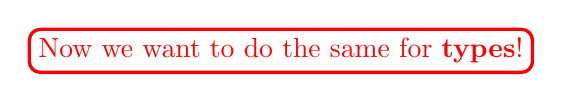
\begin{tikzpicture}
			\onslide<2>{
				\node[rounded corners, Red, draw, very thick] at (0,0) {Now we want to do the same for \textbf{types}!};
			}
		\end{tikzpicture}
	\end{center}
\end{frame}

\begin{frame}{Getting classy}
	\begin{itemize}
		\item We define a new \alert{type} in Python by defining a new \alert{class}
		\item Classes and types are synonymous in Python 3
		\item Like functions, will have two ``parts'':
			\begin{itemize}
				\item A definition portion, where we define what the type is and how we can interact with it
				\item An instance portion, where we create new objects of our type to utilize in our code
					\begin{itemize}
						\item ``An instance of C'' and ``An object of type C'' are telling you the same thing.
					\end{itemize}
			\end{itemize}
	\end{itemize}
\end{frame}

%\begin{frame}{The Start of Class}
	%\begin{itemize}
		%\item Use the keyword \pyi{class} to indicate the start of a new class/type definition
		%\item The following word gives the name of the new class/type
			%\begin{itemize}
				%\item Python convention is usually to start these with a capital
				%\item Doesn't need parentheses afterwards
				%\item \pyi{class Person:}
			%\end{itemize}
	%\end{itemize}
%\end{frame}















\end{document}

